% ============================================================
% 讲义 — 人教版高二选择性必修第一册 第3章 圆锥曲线与方程
% 编译命令：xelatex -interaction=nonstopmode 高二选必1_第3章_圆锥曲线与方程.tex
% ============================================================
\documentclass[12pt, a4paper]{ctexart}
\usepackage[margin=2.2cm]{geometry}
\usepackage{amsmath, amssymb}
\usepackage{enumitem}
\usepackage{tcolorbox}
\usepackage{booktabs}
\usepackage{array}
\usepackage{fancyhdr}
\usepackage{xcolor}
\usepackage{tikz}
\usepackage{hyperref}
\usepackage{graphicx}
\usepackage{multirow}
\usepackage{pgfplots}
\pgfplotsset{compat=1.18}

% 颜色定义
\definecolor{mainblue}{RGB}{41, 98, 168}
\definecolor{lightblue}{RGB}{230, 240, 255}
\definecolor{tipgreen}{RGB}{34, 139, 87}
\definecolor{lightgreen}{RGB}{235, 250, 240}
\definecolor{warnred}{RGB}{200, 50, 50}
\definecolor{lightred}{RGB}{255, 240, 240}
\definecolor{examorange}{RGB}{210, 120, 20}
\definecolor{lightorange}{RGB}{255, 248, 235}
\definecolor{apppurple}{RGB}{120, 60, 170}
\definecolor{lightpurple}{RGB}{245, 238, 255}

% 页眉页脚
\pagestyle{fancy}
\fancyhf{}
\fancyhead[L]{\small\textcolor{mainblue}{\textbf{人教版高二选必1 · 第3章\quad 圆锥曲线与方程}}}
\fancyhead[R]{\small\textcolor{mainblue}{圆锥曲线讲义}}
\fancyfoot[C]{\small —\ \thepage\ —}
\renewcommand{\headrulewidth}{0.6pt}
\renewcommand{\headrule}{\hbox to\headwidth{\color{mainblue}\leaders\hrule height \headrulewidth\hfill}}
\renewcommand{\footrulewidth}{0pt}

% tcolorbox 样式
\newtcolorbox{knowledgebox}[1][]{%
  colback=lightblue, colframe=mainblue,
  fonttitle=\bfseries\large, title=#1,
  arc=3mm, boxrule=0.8pt,
  left=8pt, right=8pt, top=6pt, bottom=6pt
}

\newtcolorbox{tipbox}[1][]{%
  colback=lightgreen, colframe=tipgreen,
  fonttitle=\bfseries, title=#1,
  arc=2mm, boxrule=0.6pt,
  left=6pt, right=6pt, top=4pt, bottom=4pt
}

\newtcolorbox{warnbox}[1][]{%
  colback=lightred, colframe=warnred,
  fonttitle=\bfseries, title=#1,
  arc=2mm, boxrule=0.6pt,
  left=6pt, right=6pt, top=4pt, bottom=4pt
}

\newtcolorbox{examplebox}[1][]{%
  colback=lightorange, colframe=examorange,
  fonttitle=\bfseries, title=#1,
  arc=3mm, boxrule=0.8pt,
  left=8pt, right=8pt, top=6pt, bottom=6pt
}

\newtcolorbox{appbox}[1][]{%
  colback=lightpurple, colframe=apppurple,
  fonttitle=\bfseries, title=#1,
  arc=3mm, boxrule=0.8pt,
  left=8pt, right=8pt, top=6pt, bottom=6pt
}

\setCJKmainfont{Hiragino Sans GB}
\setCJKsansfont{Heiti SC}

\begin{document}

% ============ 标题页 ============
\begin{center}
{\Huge\bfseries\textcolor{mainblue}{第3章\quad 圆锥曲线与方程}}\\[12pt]
{\Large\textcolor{gray}{讲\quad 义}}\\[8pt]
\rule{0.6\textwidth}{1pt}\\[8pt]
{\normalsize 适用：人教版\quad 高二选择性必修第一册\quad |\quad 课时：5课时}
\end{center}
\vspace{10pt}

% ============================================================
% 第一部分：知识点讲解
% ============================================================
\section*{\textcolor{mainblue}{一、知识点讲解}}

% -------------------- 3.1 椭圆 --------------------
\subsection*{3.1\quad 椭圆}

\begin{knowledgebox}[定义]
平面内与两个定点$F_1, F_2$的\textbf{距离之和}等于常数$2a$（$2a > |F_1F_2|$）的点的轨迹叫做\textbf{椭圆}。
两个定点$F_1, F_2$叫做椭圆的\textbf{焦点}，两焦点之间的距离$|F_1F_2|=2c$叫做\textbf{焦距}。
\end{knowledgebox}

\vspace{4pt}

\begin{knowledgebox}[标准方程]
设椭圆的中心在原点，焦距为$2c$，长半轴长为$a$，短半轴长为$b$，其中$b^2 = a^2 - c^2$。

\textbf{焦点在$x$轴上：}
\[\frac{x^2}{a^2} + \frac{y^2}{b^2} = 1 \quad (a > b > 0)\]
焦点为$F_1(-c, 0)$，$F_2(c, 0)$。

\textbf{焦点在$y$轴上：}
\[\frac{x^2}{b^2} + \frac{y^2}{a^2} = 1 \quad (a > b > 0)\]
焦点为$F_1(0, -c)$，$F_2(0, c)$。
\end{knowledgebox}

\begin{center}
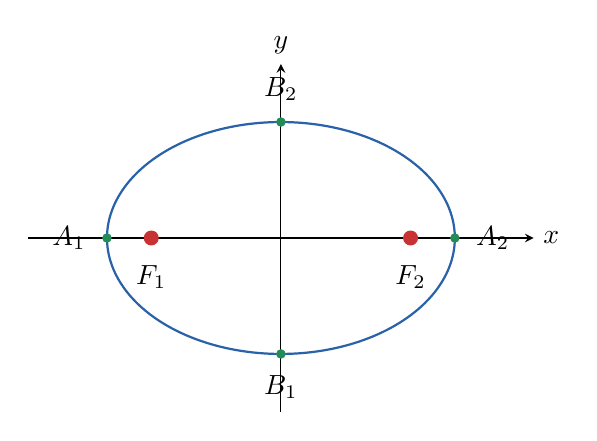
\begin{tikzpicture}
  \begin{axis}[
    width=8cm, height=6cm,
    axis equal,
    axis lines=middle,
    xlabel={$x$}, ylabel={$y$},
    xmin=-4, xmax=4, ymin=-3, ymax=3,
    ticks=none,
    every axis x label/.style={at={(current axis.right of origin)},anchor=west},
    every axis y label/.style={at={(current axis.above origin)},anchor=south},
  ]
    % 椭圆 x^2/9 + y^2/4 = 1, a=3, b=2, c=sqrt(5)
    \addplot[domain=0:360, samples=200, thick, mainblue] ({3*cos(x)},{2*sin(x)});
    % 焦点
    \addplot[only marks, mark=*, mark size=2.5pt, warnred] coordinates {({-sqrt(5)},0) ({sqrt(5)},0)};
    \node[below] at (axis cs:{sqrt(5)},-0.3) {$F_2$};
    \node[below] at (axis cs:{-sqrt(5)},-0.3) {$F_1$};
    % 顶点标记
    \addplot[only marks, mark=*, mark size=1.5pt, tipgreen] coordinates {(3,0) (-3,0) (0,2) (0,-2)};
    \node[right] at (axis cs:3.2,0) {$A_2$};
    \node[left] at (axis cs:-3.2,0) {$A_1$};
    \node[above] at (axis cs:0,2.2) {$B_2$};
    \node[below] at (axis cs:0,-2.2) {$B_1$};
  \end{axis}
\end{tikzpicture}
\end{center}

\begin{knowledgebox}[几何性质]
\renewcommand{\arraystretch}{1.4}
\begin{center}
\begin{tabular}{|l|l|}
\hline
\textbf{性质} & \textbf{内容（焦点在$x$轴）} \\
\hline
范围 & $-a \leqslant x \leqslant a$，$-b \leqslant y \leqslant b$ \\
\hline
对称性 & 关于$x$轴、$y$轴、原点对称 \\
\hline
顶点 & $(\pm a, 0)$，$(0, \pm b)$ \\
\hline
长轴长 & $2a$；短轴长 $2b$ \\
\hline
离心率 & $e = \dfrac{c}{a}$，$0 < e < 1$（越接近$0$越接近圆） \\
\hline
焦点到准线距离 & 准线 $x = \pm\dfrac{a^2}{c}$，焦准距 $= \dfrac{b^2}{c}$ \\
\hline
通径长 & $\dfrac{2b^2}{a}$（过焦点且垂直于长轴的弦） \\
\hline
\end{tabular}
\end{center}
\end{knowledgebox}

\begin{warnbox}[易错提醒]
\begin{enumerate}[leftmargin=1.5em]
  \item 椭圆标准方程中，$a$始终是\textbf{较大的分母的平方根}，$b$是较小的。判断焦点位置看哪个分母更大。
  \item $b^2 = a^2 - c^2$始终成立，不要记成$b^2 = c^2 - a^2$。
  \item 离心率$e$仅描述"扁"的程度，与椭圆大小无关。
  \item 椭圆上一点到两焦点距离之和为$2a$，这是最核心的性质。
\end{enumerate}
\end{warnbox}

% -------------------- 3.2 双曲线 --------------------
\subsection*{3.2\quad 双曲线}

\begin{knowledgebox}[定义]
平面内与两个定点$F_1, F_2$的\textbf{距离之差的绝对值}等于常数$2a$（$0 < 2a < |F_1F_2|$）的点的轨迹叫做\textbf{双曲线}。
两个定点$F_1, F_2$叫做双曲线的\textbf{焦点}，$|F_1F_2|=2c$叫做\textbf{焦距}。
\end{knowledgebox}

\vspace{4pt}

\begin{knowledgebox}[标准方程]
设双曲线的中心在原点，焦距为$2c$，实半轴长为$a$，虚半轴长为$b$，其中$b^2 = c^2 - a^2$。

\textbf{焦点在$x$轴上：}
\[\frac{x^2}{a^2} - \frac{y^2}{b^2} = 1 \quad (a > 0,\; b > 0)\]
焦点为$F_1(-c, 0)$，$F_2(c, 0)$。

\textbf{焦点在$y$轴上：}
\[\frac{y^2}{a^2} - \frac{x^2}{b^2} = 1 \quad (a > 0,\; b > 0)\]
焦点为$F_1(0, -c)$，$F_2(0, c)$。
\end{knowledgebox}

\begin{center}
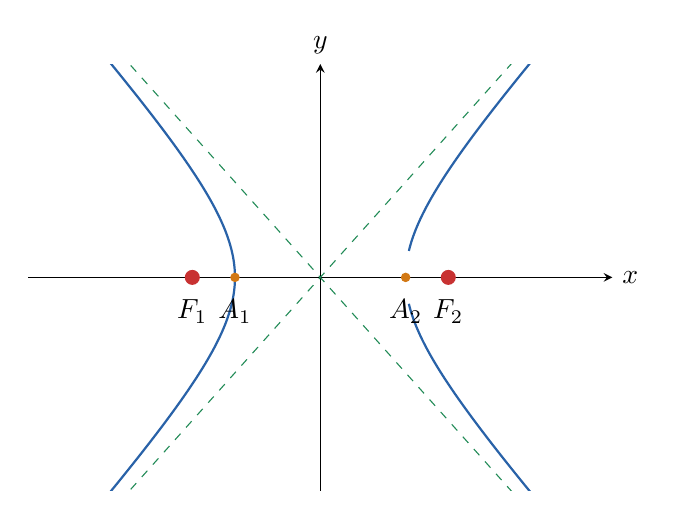
\begin{tikzpicture}
  \begin{axis}[
    width=9cm, height=7cm,
    axis equal,
    axis lines=middle,
    xlabel={$x$}, ylabel={$y$},
    xmin=-6, xmax=6, ymin=-5, ymax=5,
    ticks=none,
    every axis x label/.style={at={(current axis.right of origin)},anchor=west},
    every axis y label/.style={at={(current axis.above origin)},anchor=south},
  ]
    % 双曲线 x^2/4 - y^2/5 = 1, a=2, b=sqrt(5), c=3
    \addplot[domain=-180:-15.5, samples=200, thick, mainblue, restrict y to domain=-6:6] ({2/cos(x)},{sqrt(5)*tan(x)});
    \addplot[domain=15.5:180, samples=200, thick, mainblue, restrict y to domain=-6:6] ({2/cos(x)},{sqrt(5)*tan(x)});
    % 渐近线
    \addplot[domain=-6:6, samples=50, thin, dashed, tipgreen] ({x},{sqrt(5)/2*x});
    \addplot[domain=-6:6, samples=50, thin, dashed, tipgreen] ({x},{-sqrt(5)/2*x});
    % 焦点
    \addplot[only marks, mark=*, mark size=2.5pt, warnred] coordinates {(-3,0) (3,0)};
    \node[below] at (axis cs:3,-0.3) {$F_2$};
    \node[below] at (axis cs:-3,-0.3) {$F_1$};
    % 顶点
    \addplot[only marks, mark=*, mark size=1.5pt, examorange] coordinates {(-2,0) (2,0)};
    \node[below] at (axis cs:2,-0.3) {$A_2$};
    \node[below] at (axis cs:-2,-0.3) {$A_1$};
  \end{axis}
\end{tikzpicture}
\end{center}

\begin{knowledgebox}[几何性质]
\renewcommand{\arraystretch}{1.4}
\begin{center}
\begin{tabular}{|l|l|}
\hline
\textbf{性质} & \textbf{内容（焦点在$x$轴）} \\
\hline
范围 & $x \geqslant a$ 或 $x \leqslant -a$ \\
\hline
对称性 & 关于$x$轴、$y$轴、原点对称 \\
\hline
顶点 & $(\pm a, 0)$；虚轴端点 $(0, \pm b)$ \\
\hline
实轴长 & $2a$；虚轴长 $2b$ \\
\hline
渐近线 & $y = \pm\dfrac{b}{a}x$ \\
\hline
离心率 & $e = \dfrac{c}{a}$，$e > 1$（越大开口越大） \\
\hline
焦点到准线距离 & 准线 $x = \pm\dfrac{a^2}{c}$ \\
\hline
通径长 & $\dfrac{2b^2}{a}$ \\
\hline
\end{tabular}
\end{center}
\end{knowledgebox}

\begin{tipbox}[等轴双曲线]
当$a = b$时，双曲线$\dfrac{x^2}{a^2} - \dfrac{y^2}{a^2} = 1$称为\textbf{等轴双曲线}，其渐近线为$y = \pm x$（互相垂直），离心率$e = \sqrt{2}$。
\end{tipbox}

\begin{warnbox}[易错提醒]
\begin{enumerate}[leftmargin=1.5em]
  \item 双曲线中$b^2 = c^2 - a^2$，与椭圆$b^2 = a^2 - c^2$恰好相反。
  \item 双曲线的定义是距离之\textbf{差的绝对值}为定值，不能丢掉"绝对值"。
  \item 渐近线是双曲线独有的性质，椭圆和抛物线没有渐近线。
  \item 判断焦点位置的方法：$x^2$项系数为正$\Rightarrow$焦点在$x$轴；$y^2$项系数为正$\Rightarrow$焦点在$y$轴。
\end{enumerate}
\end{warnbox}

% -------------------- 3.3 抛物线 --------------------
\subsection*{3.3\quad 抛物线}

\begin{knowledgebox}[定义]
平面内与一个定点$F$和一条定直线$l$（$F$不在$l$上）的\textbf{距离相等}的点的轨迹叫做\textbf{抛物线}。
定点$F$叫做抛物线的\textbf{焦点}，定直线$l$叫做抛物线的\textbf{准线}。
\end{knowledgebox}

\vspace{4pt}

\begin{knowledgebox}[标准方程]
设焦点到准线的距离为$p$（$p > 0$），则抛物线的四种标准方程为：

\renewcommand{\arraystretch}{1.6}
\begin{center}
\begin{tabular}{|c|c|c|c|}
\hline
\textbf{方程} & \textbf{焦点} & \textbf{准线} & \textbf{开口方向} \\
\hline
$y^2 = 2px$ & $\left(\dfrac{p}{2}, 0\right)$ & $x = -\dfrac{p}{2}$ & 向右 \\
\hline
$y^2 = -2px$ & $\left(-\dfrac{p}{2}, 0\right)$ & $x = \dfrac{p}{2}$ & 向左 \\
\hline
$x^2 = 2py$ & $\left(0, \dfrac{p}{2}\right)$ & $y = -\dfrac{p}{2}$ & 向上 \\
\hline
$x^2 = -2py$ & $\left(0, -\dfrac{p}{2}\right)$ & $y = \dfrac{p}{2}$ & 向下 \\
\hline
\end{tabular}
\end{center}
\end{knowledgebox}

\begin{center}
\begin{tikzpicture}
  \begin{axis}[
    width=8cm, height=7cm,
    axis equal,
    axis lines=middle,
    xlabel={$x$}, ylabel={$y$},
    xmin=-1, xmax=5, ymin=-3.5, ymax=3.5,
    ticks=none,
    every axis x label/.style={at={(current axis.right of origin)},anchor=west},
    every axis y label/.style={at={(current axis.above origin)},anchor=south},
  ]
    % 抛物线 y^2 = 4x, p=2
    \addplot[domain=-3.2:3.2, samples=200, thick, mainblue] ({x^2/4},{x});
    % 焦点 F(1,0)
    \addplot[only marks, mark=*, mark size=2.5pt, warnred] coordinates {(1,0)};
    \node[below right] at (axis cs:1,0) {$F(1,0)$};
    % 准线 x = -1
    \addplot[domain=-3.5:3.5, samples=2, thin, dashed, tipgreen] ({-1},{x});
    \node[left] at (axis cs:-1,2.8) {$l:\; x=-1$};
    % 顶点
    \addplot[only marks, mark=*, mark size=1.5pt, examorange] coordinates {(0,0)};
    \node[below left] at (axis cs:0,0) {$O$};
  \end{axis}
\end{tikzpicture}
\end{center}

\begin{knowledgebox}[几何性质（以$y^2 = 2px$为例）]
\renewcommand{\arraystretch}{1.4}
\begin{center}
\begin{tabular}{|l|l|}
\hline
\textbf{性质} & \textbf{内容} \\
\hline
范围 & $x \geqslant 0$，$y \in \mathbb{R}$ \\
\hline
对称性 & 关于$x$轴对称 \\
\hline
顶点 & 原点$(0,0)$ \\
\hline
离心率 & $e = 1$ \\
\hline
焦点弦 & 过焦点弦长 $= x_1 + x_2 + p$ \\
\hline
通径长 & $2p$（过焦点且垂直于对称轴的弦） \\
\hline
\end{tabular}
\end{center}
\end{knowledgebox}

\begin{warnbox}[易错提醒]
\begin{enumerate}[leftmargin=1.5em]
  \item 方程$y^2 = 2px$中，$p > 0$，$2p$是焦点到准线的距离的\textbf{两倍}，不要混淆。
  \item 抛物线上任意一点到焦点的距离等于到准线的距离，这是最核心的性质。
  \item 抛物线只有一个焦点、一条准线，离心率恒为$1$。
  \item 焦点弦（过焦点的弦）的弦长公式：设端点横坐标为$x_1, x_2$，则$|AB| = x_1 + x_2 + p$。
\end{enumerate}
\end{warnbox}

% -------------------- 3.4 直线与圆锥曲线 --------------------
\subsection*{3.4\quad 直线与圆锥曲线的位置关系}

\begin{knowledgebox}[基本方法——联立方程法]
判断直线$l: y = kx + m$与圆锥曲线$C$的位置关系的步骤：
\begin{enumerate}[leftmargin=1.5em]
  \item 联立直线方程与圆锥曲线方程，消去$y$（或$x$），得到关于$x$（或$y$）的一元二次方程；
  \item 计算判别式$\Delta = b^2 - 4ac$；
  \item 根据$\Delta$的符号判断：
  \begin{itemize}
    \item $\Delta > 0$：直线与曲线有\textbf{两个}不同交点（相交）；
    \item $\Delta = 0$：直线与曲线有\textbf{一个}交点（相切，特殊情况为$\Delta = 0$不保证相切）；
    \item $\Delta < 0$：直线与曲线\textbf{无}交点（相离）。
  \end{itemize}
\end{enumerate}
\end{knowledgebox}

\vspace{4pt}

\begin{knowledgebox}[弦长公式]
设直线$y = kx + m$与圆锥曲线交于$A(x_1, y_1)$，$B(x_2, y_2)$两点，
联立后得到$ax^2 + bx + c = 0$，由韦达定理：$x_1 + x_2 = -\dfrac{b}{a}$，$x_1 x_2 = \dfrac{c}{a}$。

弦长公式：
\[|AB| = \sqrt{1 + k^2} \cdot |x_1 - x_2| = \sqrt{1 + k^2} \cdot \frac{\sqrt{\Delta}}{|a|}\]
其中$\Delta$为联立方程的判别式。
\end{knowledgebox}

\vspace{4pt}

\begin{knowledgebox}[中点弦问题——点差法]
设弦$AB$的中点为$M(x_0, y_0)$，若$A, B$在椭圆$\dfrac{x^2}{a^2} + \dfrac{y^2}{b^2} = 1$上，则：
\[\frac{x_1^2}{a^2} + \frac{y_1^2}{b^2} = 1, \quad \frac{x_2^2}{a^2} + \frac{y_2^2}{b^2} = 1\]
两式相减得：
\[\frac{(x_1 - x_2)(x_1 + x_2)}{a^2} + \frac{(y_1 - y_2)(y_1 + y_2)}{b^2} = 0\]
因此斜率：
\[k_{AB} = -\frac{b^2 x_0}{a^2 y_0}\]
\end{knowledgebox}

\begin{tipbox}[面积公式]
直线与圆锥曲线所围成的三角形面积：
若直线$y = kx + m$与曲线交于$A, B$两点，原点$O$到直线的距离为$d = \dfrac{|m|}{\sqrt{1+k^2}}$，则：
\[S_{\triangle OAB} = \frac{1}{2} \cdot |AB| \cdot d = \frac{|m| \cdot \sqrt{\Delta}}{2|a|}\]
\end{tipbox}

\newpage

% ============================================================
% 第二部分：例题精讲
% ============================================================
\section*{\textcolor{examorange}{二、例题精讲}}

% ---- 例题1 ----
\begin{examplebox}[【例题1】求椭圆标准方程]
已知椭圆的焦点为$F_1(-3, 0)$，$F_2(3, 0)$，且椭圆经过点$(5, 0)$，求椭圆的标准方程。
\end{examplebox}

\textbf{解：}

由焦点坐标知$c = 3$，焦点在$x$轴上。

椭圆经过点$(5, 0)$，即$(5, 0)$是椭圆的一个顶点，故$a = 5$。

于是$b^2 = a^2 - c^2 = 25 - 9 = 16$。

$$\boxed{\dfrac{x^2}{25} + \dfrac{y^2}{16} = 1}$$

% ---- 例题2 ----
\begin{examplebox}[【例题2】椭圆离心率问题]
已知椭圆$\dfrac{x^2}{4} + \dfrac{y^2}{3} = 1$，求其离心率，并求焦点到对应准线的距离。
\end{examplebox}

\textbf{解：}

$a^2 = 4$，$b^2 = 3$，故$c^2 = a^2 - b^2 = 4 - 3 = 1$，$a = 2$，$c = 1$。

离心率$e = \dfrac{c}{a} = \dfrac{1}{2}$。

准线方程为$x = \pm\dfrac{a^2}{c} = \pm 4$。

焦点$F_1(-1, 0)$到准线$x = -4$的距离为$|-1 - (-4)| = 3$。

$$\boxed{e = \frac{1}{2}, \quad \text{焦点到准线距离为}\; 3}$$

% ---- 例题3 ----
\begin{examplebox}[【例题3】求双曲线标准方程]
已知双曲线的渐近线为$y = \pm \dfrac{3}{4}x$，且经过点$(8, 3\sqrt{3})$，求双曲线的标准方程。
\end{examplebox}

\textbf{解：}

渐近线$y = \pm\dfrac{3}{4}x$，设双曲线为$\dfrac{x^2}{16} - \dfrac{y^2}{9} = \lambda$（$\lambda \neq 0$）。

代入点$(8, 3\sqrt{3})$：

$$\frac{64}{16} - \frac{27}{9} = \lambda \implies 4 - 3 = \lambda \implies \lambda = 1$$

$$\boxed{\dfrac{x^2}{16} - \dfrac{y^2}{9} = 1}$$

% ---- 例题4 ----
\begin{examplebox}[【例题4】双曲线的离心率与渐近线]
已知双曲线$\dfrac{x^2}{a^2} - \dfrac{y^2}{b^2} = 1$（$a > 0, b > 0$）的一条渐近线方程为$y = \sqrt{3}\,x$，求该双曲线的离心率。
\end{examplebox}

\textbf{解：}

渐近线$y = \pm\dfrac{b}{a}x$，由已知$\dfrac{b}{a} = \sqrt{3}$，即$b = \sqrt{3}\,a$。

$$c^2 = a^2 + b^2 = a^2 + 3a^2 = 4a^2 \implies c = 2a$$

$$e = \frac{c}{a} = 2$$

$$\boxed{e = 2}$$

% ---- 例题5 ----
\begin{examplebox}[【例题5】抛物线焦点弦问题]
过抛物线$y^2 = 4x$的焦点$F$作一条倾斜角为$60°$的弦$AB$，求弦长$|AB|$。
\end{examplebox}

\textbf{解：}

抛物线$y^2 = 4x$，$2p = 4$，$p = 2$，焦点$F(1, 0)$。

设直线方程为$y = \tan 60° \cdot (x - 1) = \sqrt{3}(x - 1)$。

代入$y^2 = 4x$：

$$3(x - 1)^2 = 4x \implies 3x^2 - 6x + 3 = 4x \implies 3x^2 - 10x + 3 = 0$$

设$A(x_1, y_1)$，$B(x_2, y_2)$，由韦达定理：

$$x_1 + x_2 = \frac{10}{3}, \quad x_1 x_2 = 1$$

焦点弦长$|AB| = x_1 + x_2 + p = \dfrac{10}{3} + 2 = \dfrac{16}{3}$。

$$\boxed{|AB| = \dfrac{16}{3}}$$

% ---- 例题6 ----
\begin{examplebox}[【例题6】直线与椭圆相交——弦长计算]
已知椭圆$\dfrac{x^2}{4} + y^2 = 1$，直线$l: y = x + 1$与椭圆交于$A, B$两点，求$|AB|$。
\end{examplebox}

\textbf{解：}

联立方程：
$$\begin{cases} \dfrac{x^2}{4} + y^2 = 1 \\ y = x + 1 \end{cases}$$

代入消去$y$：

$$\frac{x^2}{4} + (x+1)^2 = 1 \implies x^2 + 4(x^2 + 2x + 1) = 4 \implies 5x^2 + 8x = 0$$

$$x(5x + 8) = 0 \implies x_1 = 0, \quad x_2 = -\frac{8}{5}$$

$$|x_1 - x_2| = \frac{8}{5}$$

$$|AB| = \sqrt{1 + 1^2} \cdot \frac{8}{5} = \frac{8\sqrt{2}}{5}$$

$$\boxed{|AB| = \dfrac{8\sqrt{2}}{5}}$$

% ---- 例题7 ----
\begin{examplebox}[【例题7】直线与抛物线相切——求切线方程]
求过点$(1, -2)$且与抛物线$y^2 = 8x$相切的直线方程。
\end{examplebox}

\textbf{解：}

设切线方程为$y + 2 = k(x - 1)$，即$y = kx - k - 2$。

代入$y^2 = 8x$：

$$(kx - k - 2)^2 = 8x$$

$$k^2 x^2 - 2k(k+2)x + (k+2)^2 = 8x$$

$$k^2 x^2 - [2k(k+2) + 8]x + (k+2)^2 = 0$$

令$\Delta = 0$（相切条件）：

$$[2k(k+2) + 8]^2 - 4k^2(k+2)^2 = 0$$

设$m = 2k(k+2)$，则：

$$(m + 8)^2 - 4k^2(k+2)^2 = 0 \implies (m+8)^2 = m^2$$

$$m^2 + 16m + 64 = m^2 \implies 16m = -64 \implies m = -4$$

$$2k(k+2) = -4 \implies k^2 + 2k + 2 = 0$$

判别式$4 - 8 = -4 < 0$，无实数解。

因此点$(1, -2)$处不存在斜率存在的切线。检验$x = 1$是否为切线：代入抛物线$y^2 = 8$，$y = \pm 2\sqrt{2} \neq -2$，不是切线。

考虑抛物线$y^2 = 8x$的参数形式，$y = -2$代入得$x = \dfrac{1}{2}$，故点$(1, -2)$不在抛物线上。

验证点$(1, -2)$在抛物线外（$(-2)^2 = 4 < 8 \times 1 = 8$，故在内部）。

重新求解：当$k \neq 0$时上述过程已给出无解；当$k = 0$时，$y = -2$代入$y^2 = 8x$得$x = \dfrac{1}{2}$，与$x = 1$矛盾，不是切线。

实际上应设切线为$x = ty + m$形式代入，但此处最直接的方法是利用抛物线的切线公式。

\textbf{另解：}设切点为$(x_0, y_0)$在$y^2 = 8x$上，则切线方程为$y_0 y = 4(x + x_0)$。

代入$(1, -2)$：$-2y_0 = 4(1 + x_0)$，即$y_0 = -2 - 2x_0$。

又$y_0^2 = 8x_0$，代入：$(2 + 2x_0)^2 = 8x_0$，$4 + 8x_0 + 4x_0^2 = 8x_0$，$4x_0^2 + 4 = 0$，无实数解。

因此，点$(1, -2)$在抛物线内部，不存在过该点的切线。

$$\boxed{\text{不存在过点}(1,-2)\text{与抛物线}y^2=8x\text{相切的直线}}$$

\begin{warnbox}[方法总结]
判断点与抛物线的位置关系：将点代入$y^2 - 8x$，若$< 0$则在内部（不能做切线），若$= 0$则在曲线上，若$> 0$则在外部（可做两条切线）。
\end{warnbox}

% ---- 例题8 ----
\begin{examplebox}[【例题8】中点弦问题（点差法）]
已知椭圆$\dfrac{x^2}{16} + \dfrac{y^2}{4} = 1$，弦$AB$的中点为$M(2, 1)$，求弦$AB$所在直线的方程。
\end{examplebox}

\textbf{解：}

设$A(x_1, y_1)$，$B(x_2, y_2)$，中点$M(2, 1)$。

由点差法：
$$\frac{x_1^2}{16} + \frac{y_1^2}{4} = 1, \quad \frac{x_2^2}{16} + \frac{y_2^2}{4} = 1$$

两式相减：
$$\frac{x_1^2 - x_2^2}{16} + \frac{y_1^2 - y_2^2}{4} = 0$$

$$\frac{(x_1+x_2)(x_1-x_2)}{16} + \frac{(y_1+y_2)(y_1-y_2)}{4} = 0$$

$x_1 + x_2 = 4$，$y_1 + y_2 = 2$，代入：

$$\frac{4(x_1 - x_2)}{16} + \frac{2(y_1 - y_2)}{4} = 0$$

$$\frac{x_1 - x_2}{4} + \frac{y_1 - y_2}{2} = 0 \implies k_{AB} = \frac{y_1 - y_2}{x_1 - x_2} = -\frac{1}{2}$$

直线方程：$y - 1 = -\dfrac{1}{2}(x - 2)$，即$x + 2y - 4 = 0$。

$$\boxed{x + 2y - 4 = 0}$$

% ---- 例题9 ----
\begin{examplebox}[【例题9】直线与椭圆交点的面积问题]
已知椭圆$\dfrac{x^2}{4} + y^2 = 1$，直线$l: y = kx$与椭圆交于$A, B$两点（$A$在第一象限），若$\triangle AOB$的面积为$1$（$O$为原点），求$k$的值。
\end{examplebox}

\textbf{解：}

联立$y = kx$和$\dfrac{x^2}{4} + y^2 = 1$：

$$\frac{x^2}{4} + k^2 x^2 = 1 \implies x^2 = \frac{4}{1 + 4k^2}$$

$$x = \pm\frac{2}{\sqrt{1 + 4k^2}}$$

由对称性，$A$和$B$关于原点对称，设$A\left(\dfrac{2}{\sqrt{1+4k^2}},\; \dfrac{2k}{\sqrt{1+4k^2}}\right)$。

$O$到直线$kx - y = 0$的距离为$0$（直线过原点），所以用坐标公式求面积：

$$S_{\triangle AOB} = \frac{1}{2}|x_A \cdot y_B - x_B \cdot y_A| = \frac{1}{2} \cdot 2|x_A y_B - x_B y_A|$$

由于$B = -A$，$x_B = -x_A$，$y_B = -y_A$：

$$S = \frac{1}{2}|x_A(-y_A) - (-x_A)y_A| = \frac{1}{2} \cdot 2|x_A y_A| = |x_A y_A|$$

$$= \frac{2}{\sqrt{1+4k^2}} \cdot \frac{2k}{\sqrt{1+4k^2}} = \frac{4k}{1+4k^2} = 1$$

$$4k = 1 + 4k^2 \implies 4k^2 - 4k + 1 = 0 \implies (2k - 1)^2 = 0 \implies k = \frac{1}{2}$$

验证：$k = \dfrac{1}{2}$时，$A$在第一象限，满足题意。

$$\boxed{k = \dfrac{1}{2}}$$

% ---- 例题10 ----
\begin{examplebox}[【例题10】椭圆焦点三角形的面积]
已知椭圆$\dfrac{x^2}{25} + \dfrac{y^2}{9} = 1$，$F_1, F_2$为焦点，$P$为椭圆上一点，$\angle F_1 P F_2 = \dfrac{\pi}{3}$，求$\triangle F_1 P F_2$的面积。
\end{examplebox}

\textbf{解：}

$a = 5$，$b = 3$，$c = \sqrt{25 - 9} = 4$。

设$|PF_1| = r_1$，$|PF_2| = r_2$，则$r_1 + r_2 = 2a = 10$。

$|F_1 F_2| = 2c = 8$。

由余弦定理：
$$|F_1 F_2|^2 = r_1^2 + r_2^2 - 2r_1 r_2 \cos\frac{\pi}{3}$$

$$64 = r_1^2 + r_2^2 - r_1 r_2 = (r_1 + r_2)^2 - 3r_1 r_2 = 100 - 3r_1 r_2$$

$$r_1 r_2 = 12$$

$$S_{\triangle} = \frac{1}{2} r_1 r_2 \sin\frac{\pi}{3} = \frac{1}{2} \times 12 \times \frac{\sqrt{3}}{2} = 3\sqrt{3}$$

$$\boxed{S_{\triangle F_1 P F_2} = 3\sqrt{3}}$$

% ---- 例题11 ----
\begin{examplebox}[【例题11】直线与双曲线的位置关系]
判断直线$y = x + 1$与双曲线$\dfrac{x^2}{4} - y^2 = 1$的交点个数，并求交点坐标。
\end{examplebox}

\textbf{解：}

联立方程：
$$\begin{cases} \dfrac{x^2}{4} - y^2 = 1 \\ y = x + 1 \end{cases}$$

代入：
$$\frac{x^2}{4} - (x+1)^2 = 1 \implies x^2 - 4(x^2 + 2x + 1) = 4$$

$$x^2 - 4x^2 - 8x - 4 = 4 \implies -3x^2 - 8x - 8 = 0 \implies 3x^2 + 8x + 8 = 0$$

$$\Delta = 64 - 96 = -32 < 0$$

$\Delta < 0$，方程无实数根，直线与双曲线无交点。

$$\boxed{\text{直线与双曲线无交点}}$$

% ---- 例题12 ----
\begin{examplebox}[【例题12】抛物线上的点到焦点的距离]
已知抛物线$y^2 = 8x$上一点$P$到焦点$F$的距离为$6$，求点$P$的坐标。
\end{examplebox}

\textbf{解：}

抛物线$y^2 = 8x$，$2p = 8$，$p = 4$，焦点$F(2, 0)$，准线$x = -2$。

设$P(x_0, y_0)$，由抛物线定义：$|PF| = x_0 + \dfrac{p}{2} = x_0 + 2$。

$$x_0 + 2 = 6 \implies x_0 = 4$$

代入$y^2 = 8x$：$y_0^2 = 32$，$y_0 = \pm 4\sqrt{2}$。

$$\boxed{P(4, \; 4\sqrt{2}) \;\text{或}\; P(4, \; -4\sqrt{2})}$$

\newpage

% ============================================================
% 第三部分：应用题
% ============================================================
\section*{\textcolor{apppurple}{三、应用题}}

% ---- 应用1 ----
\begin{appbox}[【应用1】天体运行轨道]
一颗人造地球卫星的运行轨道是一个椭圆，地球位于椭圆的一个焦点上。已知卫星轨道的长半轴长为$a = 8000\;\text{km}$，短半轴长为$b = 7900\;\text{km}$。
\begin{enumerate}[leftmargin=1.5em]
  \item 求卫星轨道的离心率（精确到$0.001$）；
  \item 求卫星运行到近地点和远地点时与地球中心的距离。
\end{enumerate}
\end{appbox}

\textbf{解：}

\textbf{(1)}

$$c = \sqrt{a^2 - b^2} = \sqrt{8000^2 - 7900^2} = \sqrt{(8000+7900)(8000-7900)} = \sqrt{15900 \times 100}$$

$$= \sqrt{1590000} = 100\sqrt{159} \approx 100 \times 12.610 = 1261.0 \;\text{km}$$

$$e = \frac{c}{a} = \frac{1261.0}{8000} \approx 0.158$$

\textbf{(2)}

近地点距离 $= a - c = 8000 - 1261 = 6739\;\text{km}$。

远地点距离 $= a + c = 8000 + 1261 = 9261\;\text{km}$。

$$\boxed{e \approx 0.158, \quad \text{近地点}\; 6739\;\text{km}, \quad \text{远地点}\; 9261\;\text{km}}$$

% ---- 应用2 ----
\begin{appbox}[【应用2】卫星接收天线的抛物面]
某卫星接收天线的纵截面为抛物线形状，口径（两端点间的距离）为$4\;\text{m}$，深度（顶点到口径中点的距离）为$1\;\text{m}$。建立适当的坐标系，求抛物线的方程，并计算焦点到顶点的距离（即馈源的安装位置）。
\end{appbox}

\textbf{解：}

以抛物线顶点为原点，对称轴为$x$轴建立坐标系。

设抛物线方程为$y^2 = 2px$（$p > 0$）。

口径的两端点坐标为$(1, 2)$和$(1, -2)$（深度$1\;\text{m}$，口径$4\;\text{m}$，半口径$2\;\text{m}$）。

代入$(1, 2)$：$4 = 2p \times 1 = 2p$，$p = 2$。

抛物线方程为$y^2 = 4x$。

焦点到顶点的距离为$\dfrac{p}{2} = 1\;\text{m}$。

$$\boxed{y^2 = 4x, \quad \text{焦点到顶点距离}\; 1\;\text{m}}$$

% ---- 应用3 ----
\begin{appbox}[【应用3】油罐车横截面问题]
某油罐车的横截面近似为一个椭圆，长轴长$2.4\;\text{m}$，短轴长$1.8\;\text{m}$。油面距底部$0.6\;\text{m}$时，求油面的宽度。
\end{appbox}

\textbf{解：}

以椭圆中心为原点建立坐标系，长轴在$x$轴上。

$a = 1.2\;\text{m}$，$b = 0.9\;\text{m}$，椭圆方程：

$$\frac{x^2}{1.44} + \frac{y^2}{0.81} = 1$$

底部对应$y = -0.9$，油面距底部$0.6\;\text{m}$，故油面对应$y = -0.9 + 0.6 = -0.3$。

代入$y = -0.3$：

$$\frac{x^2}{1.44} + \frac{0.09}{0.81} = 1 \implies \frac{x^2}{1.44} = 1 - \frac{1}{9} = \frac{8}{9}$$

$$x^2 = 1.44 \times \frac{8}{9} = 1.28 \implies x = \pm\sqrt{1.28} \approx \pm 1.131\;\text{m}$$

油面宽度 $= 2 \times 1.131 \approx 2.26\;\text{m}$。

$$\boxed{\text{油面宽度约}\; 2.26\;\text{m}}$$

% ---- 应用4 ----
\begin{appbox}[【应用4】光学性质应用——椭圆镜面反射]
椭圆具有光学性质：从一个焦点发出的光线经椭圆反射后必经过另一个焦点。现有一个椭圆形镜面，方程为$\dfrac{x^2}{25} + \dfrac{y^2}{9} = 1$，从焦点$F_1$发出的光线射到椭圆上点$P(3, \frac{12}{5})$处，求反射光线的方程（即光线经过$F_2$的直线方程）。
\end{appbox}

\textbf{解：}

$a = 5$，$b = 3$，$c = 4$。

$F_1(-4, 0)$，$F_2(4, 0)$。

验证$P$在椭圆上：$\dfrac{9}{25} + \dfrac{144/25}{9} = \dfrac{9}{25} + \dfrac{16}{25} = 1$，成立。

由椭圆光学性质，反射光线经过$F_2(4, 0)$。

反射光线的直线经过$P(3, \frac{12}{5})$和$F_2(4, 0)$：

斜率$k = \dfrac{0 - \frac{12}{5}}{4 - 3} = -\dfrac{12}{5}$。

直线方程：$y - 0 = -\dfrac{12}{5}(x - 4)$，即$12x + 5y - 48 = 0$。

$$\boxed{12x + 5y - 48 = 0}$$

\newpage

% ============================================================
% 第四部分：课堂练习
% ============================================================
\section*{\textcolor{tipgreen}{四、课堂练习}}

\begin{enumerate}[leftmargin=1.5em]

\item 已知椭圆的两个焦点为$F_1(0, -3)$，$F_2(0, 3)$，椭圆上一点到两焦点的距离之和为$10$，求椭圆的标准方程。

\item 已知双曲线$\dfrac{x^2}{9} - \dfrac{y^2}{16} = 1$，求其焦点坐标、渐近线方程和离心率。

\item 求抛物线$x^2 = -6y$的焦点坐标和准线方程。

\item 已知椭圆$\dfrac{x^2}{5} + y^2 = 1$，直线$l$经过点$M(1, 0)$且斜率为$1$，求直线$l$与椭圆的交点坐标。

\item 已知双曲线$\dfrac{x^2}{4} - \dfrac{y^2}{3} = 1$，$F_1$为左焦点，$P$为双曲线上一点，$|PF_1| = 5$，求$|PF_2|$。

\item 过抛物线$y^2 = 2x$的焦点作弦$AB$，若$A(x_1, y_1)$，$B(x_2, y_2)$，求$x_1 x_2$的值。

\item 已知椭圆$\dfrac{x^2}{a^2} + \dfrac{y^2}{b^2} = 1$（$a > b > 0$）的离心率为$\dfrac{\sqrt{3}}{2}$，且过点$(1, \frac{3}{2})$，求椭圆方程。

\item 判断直线$y = 2x + m$与椭圆$\dfrac{x^2}{4} + y^2 = 1$相切时$m$的值。

\end{enumerate}

\vspace{12pt}

\begin{knowledgebox}[参考答案]

\textbf{1.} $c = 3$，$2a = 10$，$a = 5$，$b^2 = 25 - 9 = 16$。焦点在$y$轴上。

$$\boxed{\dfrac{x^2}{16} + \dfrac{y^2}{25} = 1}$$

\vspace{6pt}

\textbf{2.} $a^2 = 9$，$b^2 = 16$，$c = \sqrt{9+16} = 5$。

焦点：$F_1(-5, 0)$，$F_2(5, 0)$。

渐近线：$y = \pm\dfrac{4}{3}x$。

离心率：$e = \dfrac{5}{3}$。

\vspace{6pt}

\textbf{3.} $2p = 6$，$p = 3$。

焦点：$\left(0, -\dfrac{3}{2}\right)$。

准线：$y = \dfrac{3}{2}$。

\vspace{6pt}

\textbf{4.} 直线$l: y = x - 1$，联立$\dfrac{x^2}{5} + (x-1)^2 = 1$：

$$x^2 + 5x^2 - 10x + 5 = 5 \implies 6x^2 - 10x = 0 \implies x(6x - 10) = 0$$

$x_1 = 0$，$y_1 = -1$；$x_2 = \dfrac{5}{3}$，$y_2 = \dfrac{2}{3}$。

交点为$(0, -1)$和$\left(\dfrac{5}{3}, \dfrac{2}{3}\right)$。

\vspace{6pt}

\textbf{5.} $a = 2$，$c = \sqrt{4+3} = \sqrt{7}$。

由双曲线定义：$||PF_1| - |PF_2|| = 2a = 4$。

$|PF_2| = 5 + 4 = 9$（$P$在左支）或$|PF_2| = 5 - 4 = 1$（$P$在右支）。

因为$|PF_1| = 5$，左焦点到左支顶点距离为$c - a = \sqrt{7} - 2 > 0$，$P$在右支时$|PF_1| \geqslant c - a + 2a = \sqrt{7} + 2 \approx 4.65 < 5$，两种都可能。

$$\boxed{|PF_2| = 9 \;\text{或}\; |PF_2| = 1}$$

\vspace{6pt}

\textbf{6.} $p = 1$，焦点$\left(\dfrac{1}{2}, 0\right)$。

$$x_1 x_2 = \frac{p^2}{4} = \frac{1}{4}$$

\vspace{6pt}

\textbf{7.} $e = \dfrac{c}{a} = \dfrac{\sqrt{3}}{2}$，$c^2 = \dfrac{3}{4}a^2$，$b^2 = a^2 - c^2 = \dfrac{1}{4}a^2$。

代入$(1, \frac{3}{2})$：$\dfrac{1}{a^2} + \dfrac{9/4}{a^2/4} = 1 \implies \dfrac{1}{a^2} + \dfrac{9}{a^2} = 1 \implies a^2 = 10$，$b^2 = \dfrac{10}{4} = \dfrac{5}{2}$。

$$\boxed{\dfrac{x^2}{10} + \dfrac{2y^2}{5} = 1}$$

\vspace{6pt}

\textbf{8.} 联立$y = 2x + m$和$\dfrac{x^2}{4} + y^2 = 1$：

$$x^2 + 4(2x+m)^2 = 4 \implies x^2 + 16x^2 + 16mx + 4m^2 = 4$$

$$17x^2 + 16mx + 4m^2 - 4 = 0$$

令$\Delta = 0$：$256m^2 - 4 \times 17 \times (4m^2 - 4) = 0$

$$256m^2 - 272m^2 + 272 = 0 \implies -16m^2 + 272 = 0 \implies m^2 = 17$$

$$\boxed{m = \pm\sqrt{17}}$$

\end{knowledgebox}

\vfill
\begin{center}
\small\textcolor{gray}{本讲义仅供教学参考，例题可根据学生水平调整难度。}
\end{center}

\end{document}
